\documentclass[12pt, a4]{article}
\usepackage[english]{babel}
\usepackage[utf8x]{inputenc}
\usepackage{fullpage}
\usepackage{listings}
\usepackage{graphicx}
\usepackage{color}

%Syntax highlighting
\definecolor{blue-violet}{rgb}{0.54, 0.17, 0.89}
\definecolor{ao}{rgb}{0.0, 0.5, 0.0}
\definecolor{amaranth}{rgb}{0.9, 0.17, 0.31}
\definecolor{ballblue}{rgb}{0.13, 0.67, 0.8}
\definecolor{onyx}{rgb}{0.06, 0.06, 0.06}


\lstset{
  breaklines=true,                 % automatic line breaking only at whitespace
  captionpos=b,                    % sets the caption-position to bottom
  breakatwhitespace=false,
  keepspaces=true,
  numbers=left,
  numbersep=5pt,
  showspaces=false,
  showstringspaces=false,
  showtabs=false,
  tabsize=4,  
  backgroundcolor=\color{white},   % choose the background color
  commentstyle=\color{ao},    % comment style
  keywordstyle=\color{amaranth},    % keyword style
  stringstyle=\color{blue-violet},    % string literal style
  numberstyle=\tiny\color{ballblue},	   % number style
  basicstyle=\ttfamily\footnotesize\color{onyx} % size of fonts used for the code
}

%Document Header
\title{\textbf{Department of CSE\\SSN College of Engineering}}
\author{\textbf{Vishakan Subramanian - 18 5001 196 - Semester VI}}
\date{20 February 2021}

\begin{document}
\maketitle
\hrule
\section*{\center{UCS 1602 - Compiler Design}}
\hrule
\bigskip

%Assignment Details
\subsection*{\center{\textbf{Exercise 3: Elimination of Left Recursion Using C}}}
\subsection*{\flushleft{Aim:}}
\begin{flushleft}
Write a program in C to find whether the given grammar is \textbf{Left Recursive} or not. If it is found to be left recursive, convert the grammar in such a way that the left recursion is removed.
\end{flushleft}

%Code
\newpage
\subsection*{\flushleft{Code:}}
\begin{flushleft}
\lstinputlisting[language = C]{LR.c}
\end{flushleft}

%Output
\newpage
\subsection*{\flushleft{Output - Left Recursive Grammar:}}
\begin{figure}[h]
\centering
\caption{Console Output for a Left Recursive Grammar.}
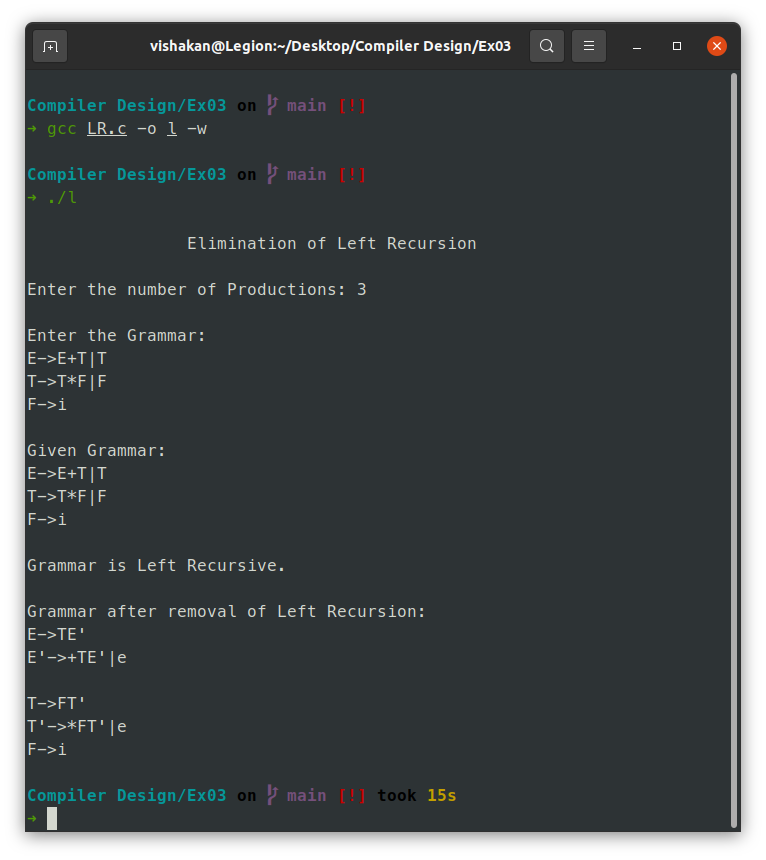
\includegraphics[scale= 0.5]{Output.png}
\end{figure}

\newpage
\subsection*{\flushleft{Output - Non Left Recursive Grammar:}}
\begin{figure}[h]
\centering
\caption{Console Output for a Non Left Recursive Grammar.}
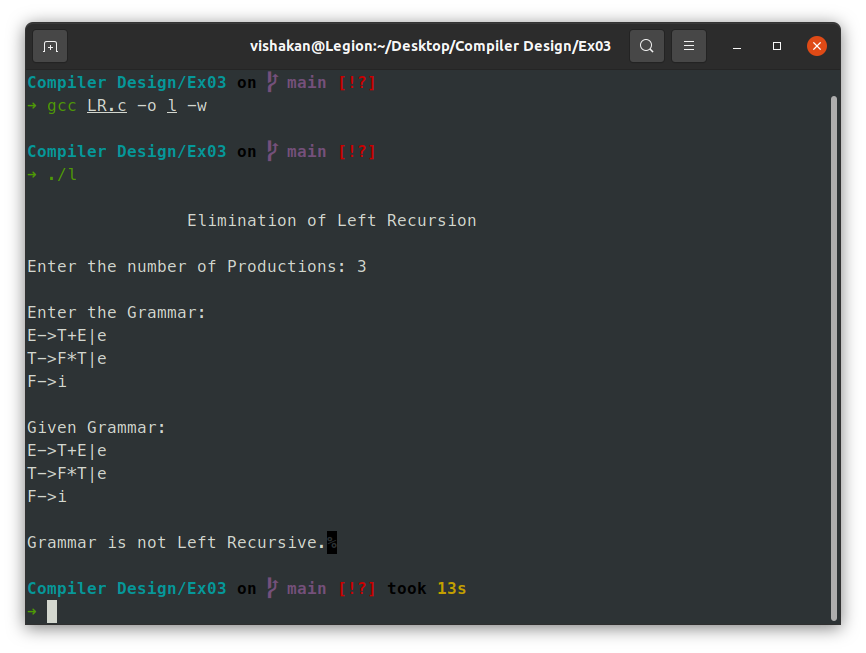
\includegraphics[scale= 0.5]{Output2.png}
\end{figure}

%Learning Outcome
\newpage
\subsection*{\flushleft{Learning Outcome:}}
\begin{itemize}

\item I understood about left recursive grammars.
\item I understood the need for this type of conversion, as top-down parsers cannot handle left recursive grammars.
\item I was able to perform a check of whether or not a grammar is left recursive using C.
\item I implemented a conversion in C which converts left recursive grammar to non left recursive grammar.
\item I refreshed my 2D-char array manipulation concepts in C.

\end{itemize}


\end{document}